\subsection{Personalize the data for each user}

The most powerful technique to ensure that your data is relevant to your users, is to customize it 
for each user. Obviously there is a trade-off here because you need some information about the user,
but if the information is transient i.e. not stored on your server, but only on the browser, then this
is not an issue. A good example of this transient customisation is persistent filtering - when the user enters
their details, you can filter the data to show information specific to those details,
such as automatically pivoting or limiting the data to the user's age, gender, location, specific interests, economic circumstance, physical characteristics etc.\\

It is possible to do very sophisticated customisation using a single page web application, and it is
even possible to store data between visits, on the browser, avoiding security and information collection issues that
we discuss elsewhere. \\

Even when it is not possible to fully customize the data, you can look for shared characteristics in subgroups of
users and provide pre-determined customisation, focusing, and filtering options.
You have to know these in advance, and hence you must have demographic information. \\

\subsubsection*{Suggested strategies} 

\begin{itemize}
  \item Consider the particular user, and find a way to filter the results that are specifically adapted to their particular moment, place and circumstance.
\end{itemize}

\subsubsection*{In the context of Aire Guru \ldots}

We are all interested in the pollution that surrounds us, since it affects our health. The website
Aire Guru has been designed to specialize in this area. For those people who are especially sensitive to air pollution,
Aire Guru shows the air pollution with respect to the six most common medical conditions that
are affected by air pollutants.\\
 
\begin{figure}[ht]
  \centering
  \subfigure[EPOC]
    {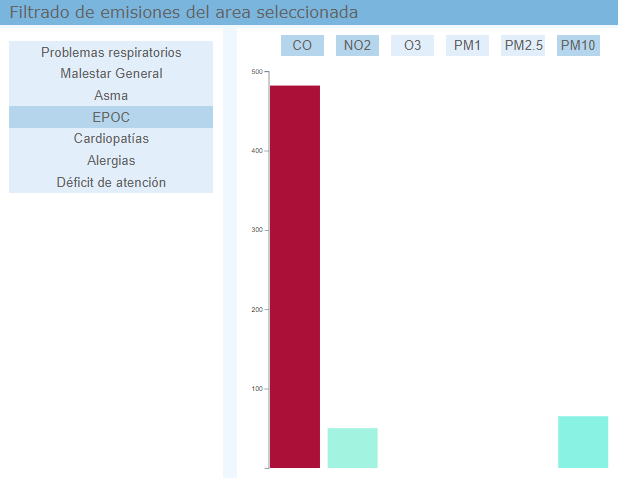
\includegraphics[width=3.5cm  ]{Figure_5_3_1_a_filter_epoc}}
  \hfill
  \subfigure [Asthma]
      {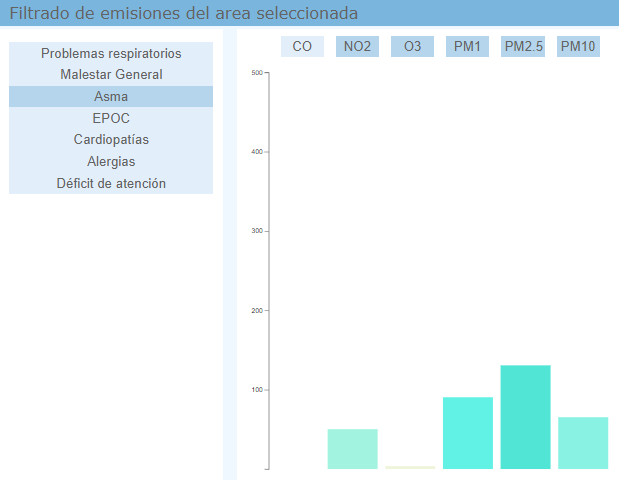
\includegraphics[width=3.5cm]{Figure_5_3_1_b_filter_asthma}}
  \hfill
  \subfigure[Allergies]
    {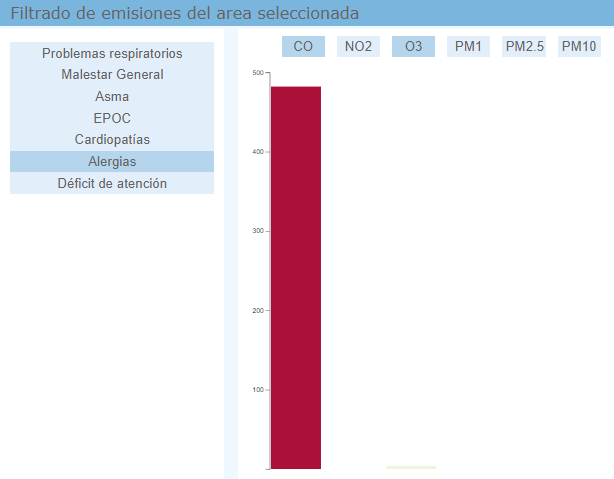
\includegraphics[width=3.5cm]{Figure_5_3_1_c_filter_allergies}}
  \caption{Medical Condition Filter}
\end{figure}

\begin{center}
  \bf{ (a)EPOC (b) Asthma (c) Allergies\\
  
  Figure 5.3.1. Medical Condition Filter}
\end{center} 

In the \textit{Figure X.X} we see, in each case, for each medical condition, a subset of pollutants which most influence each condition is shown.\\
  
The answer to the key question, how can the data be related to a specific time and place, leads us to
implementation of a personal history of exposure to pollution. That is, to know at all times what pollution
a user is subject to and where the exposure happened.\\

For this, it is essential to read the user's position. By matching the users location and the coordinates provided by the original dataset,
we can find the level of exposure to pollutants. If the user gives us his permission to store this data, we can show them their personalized history.
We implement mechanisms that provide us with the necessary security to safeguard our users data.\\

This functionality is the most powerful tool in Aire Guru. Other platforms require user-level measurement devices, i.e. the user must carry
a portable measurement station that monitors the different pollutants.\\

\begin{figure}[ht]
  \centering
  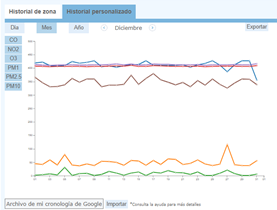
\includegraphics[width=8cm]{Figure_5_3_2_importedDataDecember}
  \caption{Personal Records. December}
\end{figure}

\begin{center}
  \bf{ 
  Figure 5.3.2. Personal Records. December}
\end{center} 

It is possible that the user may have started to use the application and not yet have any available data.
To deal with this, we have a facility to import a user's Google location history, enabling the user to visualize
exposure to pollution since the beginning of 2018 even if they have not been using the website during that period.\\

% TODO: not sure what this means
% The filtering function of the medical condition is not self-selected, because the functionality
% is available to all users. The map could show the AQI with respect to the
% pollutants that the user has preselected, but this can de-visualize the information if it is not
% clearly indicated to the user that the map does not take into account all relevant pollutants.